\documentclass[10pt, a4paper]{ReportSheet}

%%%%% Preamble with packages
%%%%% ---------------------------------------------------------------
%%%%% Encoding and fonts
%%%%% ---------------------------------------------------------------
\usepackage[utf8]{inputenc}

% hyperlinks break on hyphens
\PassOptionsToPackage{hyphens}{url}

%%%%% Other packages
%%%%% ----------------------------------------------------------------
\usepackage{amsthm}
\usepackage{bm}
\usepackage{graphicx}
\usepackage[labelfont=bf]{caption}
\newcommand{\sourceDefaultLabel}{Author's elaboration}
\newcommand{\sourceLabel}{Source:}
\newcommand{\source}[1][\sourceDefaultLabel]{\caption*{\hfill\footnotesize{\sourceLabel~\textit{#1}}}}
\usepackage{psfrag}
\usepackage{fancyvrb}
\usepackage[numbers]{natbib}
\usepackage{usebib}
\usepackage{tikz}
\usepackage{bbding}
\usepackage{icomma}
\usepackage{dcolumn}
\usepackage{booktabs}
\usepackage{paralist}
\usepackage{float}
\newcommand\foreign[1]{\emph{#1}}
\usepackage{nameref}
\newcommand{\fullref}[1]{\textbf{\nameref{#1}}}

%%%%% Color boxes
%%%%% ---------------------------------------------------------------
\usepackage{tcolorbox}
% gray box preset
\newtcolorbox{gray-box}[1]{colback=gray!5!white,colframe=gray!50!black,title=#1}
% green box preset
\newtcolorbox{green-box}[1]{
    fonttitle=\bfseries,
    coltitle=black,
    colframe=blue!20!white,
    colback=blue!5!white,
    boxrule=0mm,
    title=#1
}
% answer box
\newcommand{\answerbox}[1]{
    \begin{green-box}{\MakeUppercase{\small{Odpověď}}}
        #1
    \end{green-box}
}

\setlength{\parindent}{0pt}

%%%%% Nastavení barev a syntaxe kódu
%%%%% ---------------------------------------------------------------
\usepackage{fvextra}
\usepackage{xcolor}
\definecolor{codekeyword}{rgb}{0.0,0.3,0.7}
\definecolor{codestring}{rgb}{0.4,0.4,0.8}
\definecolor{codecomment}{rgb}{0.2,0.2,0.2}
\definecolor{codejsdoc}{rgb}{0.4,0.4,0.4}
\definecolor{codelinenum}{rgb}{0.8,0.8,0.8}
\definecolor{lightyellow}{rgb}{255, 255, 224}

% nastavení minted balíčku
\usepackage[outputdir=dist]{minted}
\setminted{
    frame=none,
    breaklines=true,
    fontsize=\footnotesize,
    tabsize=2,
    linenos,
    numbersep=5pt,
    xleftmargin=0pt,
    baselinestretch=1.2,
    style=friendly,
%   TODO: highlihgting not working
    highlightcolor=\color{lightyellow},
    keywordstyle=\color{codekeyword},
    stringstyle=\color{codestring},
    commentstyle=\color{codecomment}\itshape,
    morecomment=[s][\color{codejsdoc}]{/**}{*/},
    numberstyle=\footnotesize\color{codelinenum}
}


%%%%% Hyperlink configuration
%%%%% ------------------------------------------------------------
\hypersetup{pdftitle=MMAD - Úkol 2}

%%%%% Main document
%%%%% ------------------------------------------------------------
\begin{document}
%%% Úvod
%%% --- title, author, date
    \title{MMAD - Úkol 2}
    \author{Filip Ditrich}
    \date{
        \footnotesize{
            \centering{
                Unicorn University, Prague, Czech Republic\\
                \today
            }
        }
    }
    \maketitle

%%% Obsah
    \setcounter{tocdepth}{1}
    \pagestyle{plain}
    \renewcommand{\contentsname}{}
    \addtocontents{toc}{\vskip -2em}
    \tableofcontents

% -- TODO: Úloha 1
    \uloha{1}{2}{
        Pro následující grafy určete minimální stupeň $\delta(G)$, maximální stupeň $\Delta(G)$, skóre grafu a barevnost pro následující grafy:
        \begin{enumerate}[a]
            \item Cesta $P_n$
            \item Kružnice $C_n$
            \item Úplný graf $K_n$
            \item Úplný bipartitní graf $K_{m,n}$
            \item Papův graf ukázaný níže
        \end{enumerate}
    }{

        Nejprve si připomeneme definice:
        \begin{itemize}
            \item \textbf{Minimální stupeň $\delta(G)$} je nejmenší stupeň vrcholu v grafu $G$.
            \item \textbf{Maximální stupeň $\Delta(G)$} je největší stupeň vrcholu v grafu $G$.
            \item \textbf{Skóre grafu} je součet stupňů všech vrcholů v grafu $G$.
            \item \textbf{Barevnost} je minimální počet barev potřebných k obarvení vrcholů grafu $G$ tak, aby žádné dva sousední vrcholy neměly stejnou barvu.
        \end{itemize}
    }{false}

    \subsubsection{1a) Cesta $P_n$}
    Definice: Cesta $P_n$ je graf, který má $n$ vrcholů a $n-1$ hran.\\
    \begin{figure}[H]
        \centering
        \begin{tikzpicture}
            \node[draw, circle] (1) at (0,0) {1};
            \node[draw, circle] (2) at (1,0) {2};
            \node[draw, circle] (3) at (2,0) {3};
            \node (dots) at (3,0) {$\ldots$};
            \node[draw, circle] (n) at (4,0) {n};
            \draw (1) -- (2) -- (3) -- (dots) -- (n);
        \end{tikzpicture}
        \caption{Cesta $P_n$}
        \label{fig:ukol-2-1a-cesta}
    \end{figure}

    \answerbox{
        Uvažujme cestu $P_n$ s $n \ge 3$ vrcholy.\\
        \begin{itemize}
            \item $\delta(P_n) = 1$ ... první a poslední vrchol mají stupeň 1
            \item $\Delta(P_n) = 2$ ... všechny vrcholy kromě prvního a posledního mají stupeň 2
            \item Skóre grafu $P_n = 2n - 2$ ... vnitřní vrcholy mají stupeň 2, první a poslední vrchol mají stupeň 1
            \item Barevnost grafu $P_n = 2$ ... vždy stačí 2 barvy
        \end{itemize}
        Pro $P_2$ pak platí, že $\delta(P_2) = \Delta(P_2) = 1$.
    }{1a}

    \subsubsection{1b) Kružnice $C_n$}\\
    Definice: Kružnice $C_n$ má $n$ vrcholů a každý vrchol je spojen s předchozím a následujícím vrcholem.
    \begin{figure}[H]
        \centering
        \begin{tikzpicture}
            \node[draw, circle] (1) at (0,0) {1};
            \node[draw, circle] (2) at (1,1) {2};
            \node[draw, circle] (dots) at (2,0) {...};
            \node[draw, circle] (n) at (1,-1) {n};
            \draw (1) -- (2) -- (dots) -- (n) -- (1);
        \end{tikzpicture}
        \caption{Kružnice $C_n$}
        \label{fig:ukol-2-1b-kruznice}
    \end{figure}

    \answerbox{
        Uvažujme kružnici $C_n$ s $n \ge 3$ vrcholy.\\
        \begin{itemize}
            \item $\delta(C_n) = 2$ ... všechny vrcholy mají stupeň 2
            \item $\Delta(C_n) = 2$ ... všechny vrcholy mají stupeň 2
            \item Skóre grafu $C_n = 2n$ ... všechny vrcholy mají stupeň 2
            \item Barevnost grafu $C_n = 2$ pro sudé $n$, $3$ pro liché $n$
        \end{itemize}
    }{1b}
    \newpage

    \subsubsection{1c) Úplný graf $K_n$}\\
    Definice: Úplný graf $K_n$ má $n$ vrcholů a každý vrchol je spojen s každým jiným vrcholem.\\
    Speciální případ úplného grafu je úplný graf $K_2$, který má 2 vrcholy a 1 hranu a jedná se tedy o cestu $P_2$.\\
    Další speciální případ je úplný graf $K_3$, který má 3 vrcholy a 3 hrany a jedná se tedy o kružnici $C_3$.
    \begin{figure}[H]
        \centering
        \begin{tikzpicture}
            \node[draw, circle] (1) at (0,0) {1};
            \node[draw, circle] (2) at (2,0) {2};
            \node[draw, circle] (3) at (0,-2) {3};
            \node[draw, circle] (4) at (2,-2) {4};
            \draw (1) -- (2) -- (3) -- (4) -- (1);
            \draw (1) -- (3) -- (2) -- (4) -- (1);
        \end{tikzpicture}
        \caption{Úplný graf $K_4$}
        \label{fig:ukol-2-1c-uplny-graf}
    \end{figure}

    \answerbox{
        Uvažujme úplný graf $K_n$ s $n \ge 3$ vrcholy.\\
        \begin{itemize}
            \item $\delta(K_n) = n-1$ ... všechny vrcholy mají stupeň $n-1$
            \item $\Delta(K_n) = n-1$ ... všechny vrcholy mají stupeň $n-1$
            \item Skóre grafu $K_n = n(n-1)$ ... všechny vrcholy mají stupeň $n-1$
            \item Barevnost grafu $K_n = \begin{cases}
                                             n-1 & \text{pro sudé } n \\ n & \text{pro liché } n
            \end{cases}$
        \end{itemize}
    }{1c}

    \subsubsection{1d) Úplný bipartitní graf $K_{m,n}$}\\
    Definice: Úplný bipartitní graf $K_{m,n}$ má $m$ vrcholů v jedné partitě a $n$ vrcholů v druhé partitě a každý vrchol z jedné partity je spojen s každým vrcholem z druhé partity.

    \begin{figure}[H]
        \centering
        \begin{tikzpicture}
            \node[draw, circle] (1) at (0,0) {1};
            \node[draw, circle] (2) at (0,-1) {2};
            \node[draw, circle] (3) at (0,-2) {3};
            \node[draw, circle] (4) at (2,0) {4};
            \node[draw, circle] (5) at (2,-1) {5};
            \node[draw, circle] (6) at (2,-2) {6};
            \draw (1) -- (4);
            \draw (1) -- (5);
            \draw (1) -- (6);
            \draw (2) -- (4);
            \draw (2) -- (5);
            \draw (2) -- (6);
            \draw (3) -- (4);
            \draw (3) -- (5);
            \draw (3) -- (6);
        \end{tikzpicture}
        \caption{Úplný bipartitní graf $K_{3,3}$}
        \label{fig:ukol-2-1d-uplny-bipartitni-graf}
    \end{figure}

    \answerbox{
        Uvažujme úplný bipartitní graf $K_{m,n}$ s $m,n \ge 1$ vrcholy.\\
        \begin{itemize}
            \item $\delta(K_{m,n}) = n$ ... všechny vrcholy z první partity mají stupeň $n$
            \item $\Delta(K_{m,n}) = m$ ... všechny vrcholy z druhé partity mají stupeň $m$
            \item Skóre grafu $K_{m,n} = mn$ ... všechny vrcholy z první partity mají stupeň $n$, všechny vrcholy z druhé partity mají stupeň $m$
            \item Barevnost grafu $K_{m,n} = 2$ ... vždy stačí 2 barvy, jedna pro každou partitu
        \end{itemize}
    }{1d}
    \newpage

    \subsubsection{1e) Papův graf}\\
    Definice: Na obrázku níže je zobrazen Papův graf s 18 vrcholy a 27 hranami.\\
    \begin{figure}[H]
        \centering
        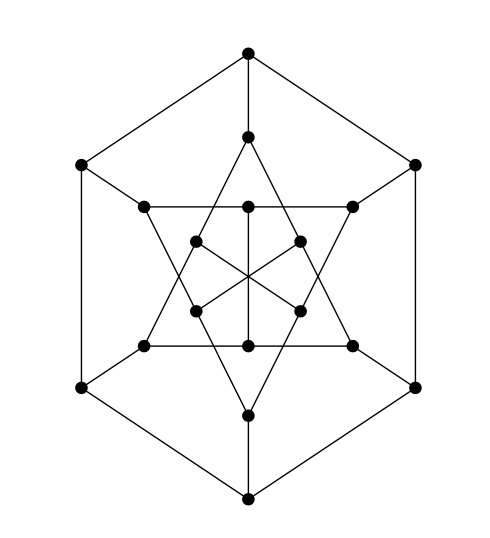
\includegraphics[width=0.35\textwidth]{\FIGDIR/ukol-2-1-papuv-graf}
        \caption{Papův graf}
        \label{fig:ukol-2-1-papuv-graf}\label{fig:figure}
    \end{figure}

    \answerbox{
        TODO:
        \begin{itemize}
            \item $\delta(\text{Papův graf}) = 3$ ... všechny vrcholy mají stupeň 3
            \item $\Delta(\text{Papův graf}) = 3$ ... všechny vrcholy mají stupeň 3
            \item Skóre grafu $\text{Papův graf} = 18 \times 3 = 54$ ... všechny vrcholy mají stupeň 3
            \item Barevnost grafu $\text{Papův graf} = TODO?$
        \end{itemize}
    }{1e}
    \newpage

% -- TODO: Úloha 2
    \uloha{2}{2}{
        Máme graf $G = (V, E)$. Pro ukázku si představme následující graf $H$:

        \begin{figure}[H]
            \centering
            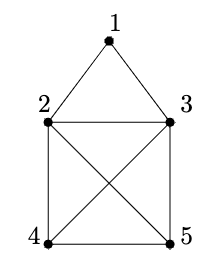
\includegraphics[width=0.2\textwidth]{\FIGDIR/ukol-2-2-graf}
            \caption{Graf $H$}
            \label{fig:ukol-2-2-graf}
        \end{figure}

        Definujme Laplacovu matici $L$ jako:

        \begin{equation*}
            L_{i,j} = \begin{cases}
                          \deg(v_i) & \text{pro } i = j \\
                          -1 & \text{pro } i \ne j \text{ a } v_i \text{ je spojen s } v_j \\
                          0 & \text{jinak}
            \end{cases}
        \end{equation*}

        Například pro ukázkový graf dostaneme Laplacovu matici:

        \begin{equation*}
            L = \begin{pmatrix}
                    2  & -1 & -1 & 0  & 0  \\
                    1  & 4  & -1 & -1 & -1 \\
                    -1 & -1 & 4  & -1 & -1 \\
                    0  & -1 & -1 & 3  & -1 \\
                    0  & -1 & -1 & -1 & 3
            \end{pmatrix}
        \end{equation*}

        Mějme $k$-regulární graf $G = (V, E)$ velikosti $|V| = n$, tj. graf pro který víme, že $\deg(v_i) = k$ pro
        všechny vrcholy $v_i \in V$. Navíc víme, že vlastní čísla matice sousednosti jsou reálná v pořadí $\lambda_1(A) \ge \lambda_2(A) \ge \ldots \ge \lambda_n(A)$. Lze nějak obecně vyjádřit všechna vlastní čísla Laplacovy matice takového grafu?
    }{TODO}{false}{false}
    \newpage

% -- Úloha 3
    \uloha{3}{2}{
        Určete minimální a maximální počet hran v grafu na $n$ vrcholech s $c$ komponentami.
    }{}{false}{true}
    Cílem je nalézt rozsah (minimální a maximální) možných hran v grafu skládajícím se z $n$ vrcholů rozdělených do $
    c$ komponent. Komponentou se rozumí podgraf, ve kterém jsou všechny vrcholy spojeny cestou a který není spojen s
    žádnými dalšími vrcholy v hlavním grafu.

    \textbf{a) Postup pro nalezení minimálního počtu hran}:
    \begin{itemize}
        \item Izolované komponenty: Minimální počet hran nastává, když mají komponenty co nejméně hran. Extrémním
        případem je mít komponenty bez hran, tedy izolované vrcholy.
        \item Neizolované komponenty: Pro každou komponentu, která není jediný izolovaný vrchol, je minimální
        struktura vlastně strom. Strom s $k$ vrcholy má $k-1$ hran (minimum pro udržení grafu spojeného).
        \item Pokud je potřeba $c$ komponent a předpokládáme že $c-1$ komponent jsou jednotlivé izolované vrcholy a jedna komponenta obsahuje zbytek vrcholů, $n-(c-1)$, tato poslední komponenta jako strom by měla $n-(c-1)-1=n-c$ hran.
        \item Minimální počet hran je tedy $0 + (n-c) = n-c$.
    \end{itemize}

    Příklad na grafu s $n=10$ vrcholy a $c=3$ komponentami:
    \begin{itemize}
        \item Izolované komponenty: 2 izolované vrcholy, 1 komponenta s 8 vrcholy.
        \item Minimální počet hran: $10 - 3 = 7$.
    \end{itemize}

    \answerbox{
        Minimální počet v grafu na $n$ vrcholech s $c$ komponentami je $n-c$.
    }{3a}

    \textbf{b) Postup pro nalezení maximálního počtu hran}:
    \begin{itemize}
        \item Maximální počet hran nastává, když každá komponenta je úplný graf (graf, kde jsou každé různé vrcholy spojeny jedinou hranou).
        \item Respektive postačí nám jedna komponenta jako úplný graf a zbytek komponent jako izolované vrcholy (tedy
        bez hran).
        \item Počet hran v úplném grafu na $k$ vrcholech je $\binom{k}{2}$
        \item Náš úplný graf má $n-(c-1)$ vrcholů, tedy počet vrcholů mínus počet ostatních izolovaných vrcholů (
        komponent).
        \item Maximální počet hran je tedy $\binom{n-(c-1)}{2}$.
    \end{itemize}

    Příklad na grafu s $n=10$ vrcholy a $c=3$ komponentami:
    \begin{itemize}
        \item Úplný graf s 8 ($10-(3-1)$) vrcholy a 1 izolovaný vrchol.
        \item Maximální počet hran: $\binom{10-2}{2} = 28$.
    \end{itemize}

    \answerbox{
        Maximální počet v grafu na $n$ vrcholech s $c$ komponentami je $\binom{n-(c-1)}{2}$.
    }{3b}
    \newpage

% -- TODO: Úloha 4
    \uloha{4}{2}{
        Mějme následující funkci:
        \begin{equation*}
            f(x, y) = 100(y - x^2)^2 + (1 - x)^2
        \end{equation*}

        Vypočtěte gradient $\nabla f(x)$ a Hessian $\nabla^2 f(x)$ a rozhodněte (a zdůvodněte)
        zda-li je v bodě $(1, 1)$ splněna 1. podmínka pro lokální minimizátor (nulovost gradientu) či zda-li je splněna i 2. podmínka pro Hessovu matici.
    }{TODO}{false}{false}
    \newpage

% -- Úloha 5
    \uloha{5}{2}{
        Mějme množinu $\{1, 2, \ldots, n\}$. Určete, kolik je možné na této množině najít různých kružnic délky $n$? (jedná se tedy o počet průchodů, ale neorientovaného grafu).
    }{}{false}{true}
    Problém můžeme řešit následovně:
    \begin{itemize}
        \item Krok 1: Seřadíme vrcholy kružnice do pořadí $1, 2, \ldots, n$. Takových sekvencí je $n!$.
        \item Krok 2: Zvolíme si jeden výchozí vrchol (symetrická rotace). Tím tedy získáme $(n-1)!$ unikátních sekvencí, ignorujeme-li rotace.
        \item Krok 3: Otočením sekvence získáme stejnou kružnici. Počet kružnic tedy musíme dělit dvěma (pro $n>2$), protože každá sekvence a její zrcadlový obraz jsou v kružnici identické.
        \item Počet různých neorientovaných kružnic délky $n$ (pro $n>2$) je tedy: $\frac{(n-1)!}{2}$.
    \end{itemize}

    \textbf{Ukázka}: na příkladu množiny $\{1, 2, 3, 4\}$:\\
    Dle definice výše víme, že počet různých neorientovaných kružnic délky $4$ bude $\frac{(4-1)!}{2} = 3$.

    A bude se jednat o tyto 3 kružnice:
    \begin{enumerate}
        \item $1 \rightarrow 2 \rightarrow 3 \rightarrow 4 \rightarrow 1$
        \item $1 \rightarrow 2 \rightarrow 4 \rightarrow 3 \rightarrow 1$
        \item $1 \rightarrow 3 \rightarrow 2 \rightarrow 4 \rightarrow 1$
    \end{enumerate}

    \begin{figure}[H]
        \centering
        \begin{tikzpicture}[scale=0.8]
            \node[circle, draw, inner sep=2pt, fill=black, label=above:{1}] (1) at (0,2) {};
            \node[circle, draw, inner sep=2pt, fill=black, label=right:{2}] (2) at (2,0) {};
            \node[circle, draw, inner sep=2pt, fill=black, label=below:{3}] (3) at (0,-2) {};
            \node[circle, draw, inner sep=2pt, fill=black, label=left:{4}] (4) at (-2,0) {};
            \draw[->,>=stealth] (1) -- (2);
            \draw[->,>=stealth] (2) -- (3);
            \draw[->,>=stealth] (3) -- (4);
            \draw[->,>=stealth] (4) -- (1);
            \node at (0,-3)
        \end{tikzpicture}
        \quad
        \begin{tikzpicture}[scale=0.8]
            \node[circle, draw, inner sep=2pt, fill=black, label=above:{1}] (1) at (0,2) {};
            \node[circle, draw, inner sep=2pt, fill=black, label=right:{2}] (2) at (2,0) {};
            \node[circle, draw, inner sep=2pt, fill=black, label=left:{4}] (4) at (-2,0) {};
            \node[circle, draw, inner sep=2pt, fill=black, label=below:{3}] (3) at (0,-2) {};
            \draw[->,>=stealth] (1) -- (2);
            \draw[->,>=stealth] (2) -- (4);
            \draw[->,>=stealth] (4) -- (3);
            \draw[->,>=stealth] (3) -- (1);
            \node at (0,-3)
        \end{tikzpicture}
        \quad
        \begin{tikzpicture}[scale=0.8]
            \node[circle, draw, inner sep=2pt, fill=black, label=above:{1}] (1) at (0,2) {};
            \node[circle, draw, inner sep=2pt, fill=black, label=right:{3}] (3) at (2,0) {};
            \node[circle, draw, inner sep=2pt, fill=black, label=below:{2}] (2) at (0,-2) {};
            \node[circle, draw, inner sep=2pt, fill=black, label=left:{4}] (4) at (-2,0) {};
            \draw[->,>=stealth] (1) -- (3);
            \draw[->,>=stealth] (3) -- (2);
            \draw[->,>=stealth] (2) -- (4);
            \draw[->,>=stealth] (4) -- (1);
            \node at (0,-3)
        \end{tikzpicture}
        \caption{Různé neorientované kružnice délky 4}
        \label{fig:ukol-2-5-kruznice}
    \end{figure}

    \answerbox{
        Pro množinu $\{1, 2, \ldots, n\}$ je možné najít $\frac{(n-1)!}{2}$ různých neorientovaných kružnic délky $n$.
    }

    \newpage

% -- TODO: Úloha 6
    \uloha{6}{2}{
        Mějme graf $G_{n,2} = (V, E)$ definovaný následovně. Množina vrcholů jsou všechny podmnožiny množiny $A = \{1, 2, \ldots, n\}$ o velikosti 2, tedy například $v_1 = \{1, 2\}, v_2 = \{2, 3\}, \ldots$. Hrany spojují ty vrcholy $v_i = \{a, b\}, v_2 = \{c, d\}$, které sdílí právě jeden prvek, tj. $a = b \ne c = d$. Příklad takového grafu je vidět na následujícím obrázku.

        \begin{figure}[H]
            \centering
            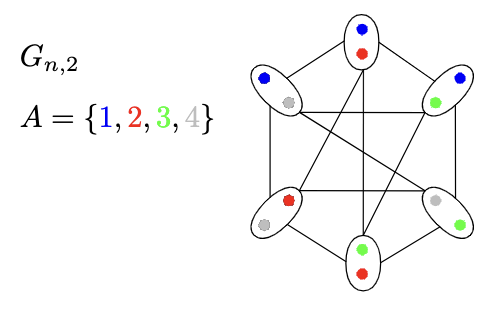
\includegraphics[width=0.5\textwidth]{\FIGDIR/ukol-2-6-graf}
            \caption{Graf $G_{n,2}$}
            \label{fig:ukol-2-6-graf}
        \end{figure}

        Pro takový obecný graf $G_{n,2}$ určete jaký bude jeho minimální a maximální stupeň vrcholu vyjádřeno jako funkce $n$
        . Také určete počet hran tohoto grafu, opět jako funkci $n$.
    }{TODO}{false}{false}
    \newpage

% -- Úloha 7
    \uloha{7}{2}{
        Zdůvodněte, proč každá hrana vrcholově 2-souvislého grafu musí ležet na kružnici.
    }{}{false}{true}
    Vrcholově 2-souvislý graf je graf, který zůstane souvislý i po odebrání libovolního vrcholu, ale po odebrání
    alespoň dvou vrcholů se může rozpadnout na více komponent vzájemně nespojených hranami, tedy nesouvislých.

    \begin{itemize}
        \item Ve vrcholově 2-souvislém grafu musí existovat alespoň dva nezávislé průchody mezi libovolnými dvěma vrcholy.
        \item Uvažujme libovolnou hranu $uv$ ve vrcholově 2-souvislém grafu.
        \item Dle vlastností vrcholové 2-souvislosti existuje další cesta z vrcholu $u$ do vrcholu $v$, která
        neobsahuje hranu $uv$.
        \item Existence této alternativní cesty mezi vrcholy $u$ a $v$, spolu s hranou $uv$, tvoří kružnici.
        \item Kružnice je vytvořena cestou z vrcholu $u$ do vrcholu $v$ přes alternativní cestu a návratem do
        vrcholu $u$ pomocí hrany $uv$.
    \end{itemize}

    \answerbox{
        Každá hrana ve vrcholově 2-souvislém grafu musí ležet na kružnici, protože definice vrcholové 2-souvislosti zaru
        čuje přítomnost alternativních cest mezi vrcholy.
    }{}

    \newpage

% -- Úloha 8
    \uloha{8}{2}{
        Určete vrcholový a hranový stupeň grafu, neboli $\alpha(G)$ a $\kappa(G)$, pro následující grafy:
        \begin{enumerate}[a]
            \item Cesta $P_n$
            \item Kružnice $C_n$
            \item Úplný graf $K_n$
            \item Úplný bipartitní graf $K_{m,n}$
        \end{enumerate}
    }{}{false}{true}

    \textbf{Definice}:
    \begin{itemize}
        \item \textbf{Vrcholový stupeň $\alpha(G)$} je minimální počet vrcholů, které je třeba odebrat, aby se graf
        rozpadl na více komponent.
        \item \textbf{Hranový stupeň $\kappa(G)$} je minimální počet hran, které je třeba odebrat, aby se graf rozpadl
        na více komponent.
    \end{itemize}

    \subsubsection{Cesta $P_n$}
    \label{subsubsec:ukol-2-8-cesta}
    \begin{itemize}
        \item Odebráním jakéhokoliv vnitřního vrcholu se cesta rozpadne na dvě komponenty. Vrcholový stupeň je tedy $\alpha(P_n) = 1$.
        \item Odebráním jakékoliv hrany se cesta rozpadne na dvě komponenty. Hranový stupeň je tedy $\kappa(P_n) = 1$.
    \end{itemize}
    \textit{Poznámka: Bereme v potaz cestu $P_n$ s $n \geq 2$ vrcholy.}
    \answerbox{
        Pro cestu $P_n$ platí $\alpha(P_n) = 1$ a $\kappa(P_n) = 1$.
    }{8a}

    \subsubsection{Kružnice $C_n$}
    \begin{itemize}
        \item Odebráním jakéhokoliv vrcholu se z kružnice stane cesta, z tvrzení výše víme že $\alpha(P_n) = 1$.
        Vrcholový stupeň je tedy $\alpha(C_n) = \alpha(P_{n-1}) + 1$.
        \item Obdobně odebráním jakýchkoliv 2 sousedních hran se kružnice rozpadne na cestu a jeden izolovaný vrchol. Hranový stupeň je tedy $\kappa(C_n) = 2$.
    \end{itemize}
    \textit{Poznámka: Bereme v potaz kružnici $C_n$ s $n \geq 3$ vrcholy.}
    \answerbox{
        Pro kružnici $C_n$ platí $\alpha(C_n) = 2$ a $\kappa(C_n) = 2$.
    }{8b}

    \subsubsection{Úplný graf $K_n$}
    \begin{itemize}
        \item Postupným odebíráním vrcholů zůstává graf stále souvislý, dokud neodebereme až $n-1$ vrcholů, pak zůstává pouze izolovaný vrchol. Vrcholový stupeň je tedy $\alpha(K_n) = n-1$.
        \item Odebráním všech hran jednoho vrcholu, který má stupeň $n-1$, se graf rozpadne jednu jednu souvislou
        komponentu a izolovaný vrchol. Hranový stupeň je tedy $\kappa(K_n) = n-1$.
    \end{itemize}
    \textit{Poznámka: Bereme v potaz úplný graf $K_n$ s $n \geq 2$ vrcholy.}
    \answerbox{
        Pro úplný graf $K_n$ platí $\alpha(K_n) = n-1$ a $\kappa(K_n) = n-1$.
    }{8c}

    \subsubsection{Úplný bipartitní graf $K_{m,n}$}
    \begin{itemize}
        \item Odebráním všech vrcholů jedné partity se graf rozpadne na několik izolovaných vrcholů (jelikož každý
        vrchol z jedné partity je spojen s každým vrcholem z druhé partity, ale nikoliv s vrcholem ze stejné partity). Lze tedy říci, že vrcholový stupeň je $\alpha(K_{m,n}) = \min(m, n)$.
        \item Odebráním všech hran spojujících vrcholy jedné partity se graf rozpadne na souvislou komponentu a
        několik izolovaných vrcholů. Pokud vybereme vrchol z větši parity, musíme odebrat pouze tolik hran, kolik
        vrcholů má menší parita, tedy opět hranový stupeň je tedy $\kappa(K_{m,
        n}) = \min(m, n)$.
    \end{itemize}
    \answerbox{
        Pro úplný bipartitní graf $K_{m,n}$ platí $\alpha(K_{m,n}) = \min(m, n)$ a $\kappa(K_{m,n}) = \min(m, n)$.
    }{8d}

    \newpage

% -- TODO: Úloha 9
    \uloha{9}{2}{
        Vezměmě si grafy typu strom o fixní velikosti $n$. Rozhodněte a nakreslete, jaký strom o velikosti $n$ má:
        \begin{enumerate}
            \item Největší hodnotu nezávislosti $\alpha(G)$
            \item Nejmenší hodnotu nezávislosti $\alpha(G)$
            \item Největší hodnotu vrcholového pokrytí $\beta(G)$
            \item Nejmenší hodnotu vrcholového pokrytí $\beta(G)$
        \end{enumerate}
    }{TODO}{false}{false}
    \newpage

% -- Úloha 10
    \uloha{10}{2}{
        Ukažte proč pro každý kubický graf $G$, t.j. takový, že všechny stupně vrcholů jsou 3, platí, že stupeň vrcholové i hranové souvislosti se rovnají, tj. $\alpha(G) = \kappa(G)$.
        \textit{Hint: Pokuste se rozebrat případy pro různé vrcholové stupně souvislosti.}
    }{}{false}{true}

    Víme, že pro každý graf $G=(V, E)$ platí \textit{Whitneyho nerovnost}:
    \begin{equation*}
        \kappa(G) \leq \alpha(G) \leq \delta(G)
    \end{equation*}
    kde $\delta(G)$ je minimální stupeň vrcholu v grafu $G$. Pro kubický graf tedy platí $\delta(G) = 3$.

    \textbf{Odebírání hran a vrcholů v kubickém grafu}:
    \begin{itemize}
        \item Odebráním hrany se sníží stupeň dvou vrcholů z 3 na 2, ale graf zůstává souvislý.
        \item Odebráním vrcholu se sníží stupeň tří hran z 3 na 2, což může vést k rozpadu grafu.
        \item Zatím můžeme pozorovat, že odebrání vrcholu může být více kritické než odebrání hrany.
    \end{itemize}

    \textbf{Případy pro různé vrcholové stupně souvislosti}:
    \begin{itemize}
        \item \textbf{Případ 1:} Pokud $\alpha(G) = 1$, graf obsahuje most, který po odebrání rozdělí graf na dvě
        komponenty. Odebráním jednoho vrcholu se graf rozpadne, tedy $\kappa(G) = 1$ také.
        \item \textbf{Případ 2:} Pokud $\alpha(G) > 1$, odebrání jednoho vrcholu nevede k rozpadu grafu, což naznačuje vyšší odolnost, tedy $\kappa(G)$ může být 2 nebo 3.
        \begin{itemize}
            \item Vzhledem k tomu, že kubické grafy mají vrcholy a hrany těsně propojeny kvůli jejich uniformnímu stupni, odebrání minimálního počtu vrcholů obvykle znamená odebrání i minimálního počtu hran.
        \end{itemize}
        \item \textbf{Případ 3:} Pro $\alpha(G) = 2$ nebo $\alpha(G) = 3$ bude kubický graf vyžadovat podobně minimální počet odebraných vrcholů k rozdělení, což znamená, že $\kappa(G)$ bude obvykle odpovídat $\alpha(G)$.
    \end{itemize}

    \answerbox{
        Díky stejnému stupni vrcholů v kubickém grafu $G$ platí, že stupeň vrcholové i hranové souvislosti jsou stejné, tj. $\alpha(G) = \kappa(G)$.
    }{}
    \newpage

% -- TODO: Úloha 11
    \uloha{11}{2}{
        Pokuste se navrhnout Turingův stroj pro rozpoznání, že neorientovaný graf má izolovaný vrchol.\\
        \textit{Hint: Graf uložte na pásku jako matici sousednosti (nezapomeňte na oddělovače řádků) a v ní pomocí pravidel nalezněte takový vrchol.}
    }{TODO}{false}{false}
    \newpage

% -- TODO: Úloha 12
    \uloha{12}{2}{
        Využijte vysvětlení proč platí polynomialita 2-SAT a nakreslete graf odpovídající následující formuli a otestujte a případně ukažte, zda-li je splněna.
        \textit{Pozn.: Graf na kreslete, i když budete schopni splnitelnost rozhodnout jinak.}

        \begin{equation*}
            f(x_1, x_2, x_3, x_4, x_5) = (x_1 \lor \overline{x_3}) \land (x_2 \lor x_3) \land (\overline{x_3} \lor x_4) \land (\overline{x_2}
            \lor
            \overline{x_4}) \land (x_4 \lor x_5) \land (\overline{x_3} \lor x_5)
        \end{equation*}
    }{TODO}{false}{false}
    \newpage

% -- TODO: Úloha 13
    \uloha{13}{2}{
        Na základě vysvětlení převodu SAT na IND nakreslete graf odpovídající následující formuli a otestujte splnitelnost formule nalezením nezávislé množiny.
        \textit{Pozn.: Graf nakreslete a zhodnoťte, i když budete schopni splnitelnost rozhodnout jinak.}

        \begin{equation*}
            f(x_1, x_2, x_3, x_4, x_5) = (x_2 \lor \overline{x_3} \lor x_4) \land (x_1 \lor \overline{x_2} \lor x_3) \land (\overline{x_1}
            \lor \overline{x_3}
            \lor
            x_4) \land (x_1 \lor \overline{x_2} \lor x_3 \lor \overline{x_4}) \land (x_4 \lor x_5)
        \end{equation*}
    }{TODO}{false}{false}
    \newpage

% -- TODO: Úloha 14
    \uloha{14}{2}{
        Na základě vysvětlení převodu 3-SAT na 3-COL nakreslete graf odpovídající následující formuli a otestujte barevnost grafu.
        \begin{equation*}
            f(x_1, x_2, x_3, x_4, x_5) = (x_1 \lor x_2 \lor \overline{x_4}) \land (x_1 \lor \overline{x_2} \lor x_3) \land (\overline{x_2}
            \lor \overline{x_3} \lor x_4) \land (x_1 \lor \overline{x_2} \lor x_3)
        \end{equation*}
    }{TODO}{false}{false}
    \newpage

% -- Úloha programovací 1
    \uloha{programovací 1}{4}{
        Naprogramujte algoritmus pro testování isomorfismu grafů hrubou silou a otestujte to na pár příkladech grafů s využitím knihovní funkce pro testování isomorfismu.
    }{}{false}{true}
    Isomorfismus lze testovat hrubou silou, kde se všechny možné permutace uzlů grafu $G$ porovnají s uzly grafu $H$.

    Vytvoříme funkci \texttt{isomorphism(G, H)}, která otestuje isomorfismus grafů $G$ a $H$ následovně:
    \begin{itemize}
        \item Pokud mají grafy různý počet uzlů, vrátí \texttt{False}.
        \item Pro všechny permutace uzlů grafu $G$:
        \begin{itemize}
            \item Vytvoří mapování uzlů grafu $G$ na uzly grafu $H$.
            \item Pokud všechny uzly grafu $G$ mají svůj ekvivalent v grafu $H$ a všechny hrany zůstanou zachovány, vrátí \texttt{True}.
        \end{itemize}
        \item Pokud žádná permutace nevyhovuje, vrátí \texttt{False}.
    \end{itemize}

    Implementačně je algoritmus následující:
    \begin{minted}{python}
        import networkx as nx
        import itertools

        def isomorphism(G, H):
            if len(G.nodes) != len(H.nodes):
                return False

            # získání všech permutací uzlů grafu G
            perms = itertools.permutations(list(G.nodes))
            for perm in perms:
                # vytvoření mapování uzlů grafu G na uzly grafu H
                # pokud všechny uzly grafu G mají svůj ekvivalent v grafu H a všechny hrany zůstanou zachovány, vrátí True
                mapping = dict(zip(G.nodes, perm))
                has_all_nodes = all([mapping[u] in H.nodes for u in G.nodes])
                has_all_edges = all([mapping[u] in H.nodes for u in G.nodes])
                if has_all_nodes and has_all_edges:
                    return True
                return False
    \end{minted}

    Poté již zbývá jen funkci výše otestovat na několika příkladech grafů a porovnat výsledky s knihovní funkcí pro
    testování isomorfismu:
    \begin{minted}{python}
        G = nx.generators.small.cycle_graph(5)
        H = nx.complement(nx.generators.small.cycle_graph(5))

        my_isom = isomorphism(G, H)
        nx_isom = nx.is_isomorphic(G, nx.complement(H))
        print(f"Vlastní: {my_isom}\nNetworkX: {nx_isom}\nÚspěch: {'Ano' if my_isom == nx_isom else 'Ne'}")
    \end{minted}

    \textit{
        Úplný zdrojový kód je k nalezení v souboru \href{https://github.com/filipditrich/MMAD-2024/blob/main/ukol-2-k1.py}{ukol-2-k1.py}.
    }
    \newpage

% -- TODO: Úloha programovací 2
    \uloha{programovací 2}{4}{
        Realizujte hrubou silou nalezení největší nezávislé množiny daného grafu a následně otestujte, že je množina nezávislá. Následně se pokuste vylepšit řešení procházení množinami použitím sousedů vrcholu.

        Pokud chceme testovat procházení, nabízí se, ne nutně, řešení pomocí nějakého rekurzivního přístupu.
    }{TODO}{false}{false}
    \newpage
\end{document}
